\section{Hardware}

\subsection{Introduction}

This section will present the hardware architecture of this project. The assembly must meet the constraints of the embedded
systems, i.e. constraints of size, weight and power consumption. As shown in
figure 1, the car is based on the Raspberry Pi 3B+ board and has a rear engine
managed by an ESC and a servo motor to control the steering at the front. Finally,
as far as sensors are concerned, we have at our disposition an \textit{Inertial Unit}, a 
\textit{Global Navigation Satellite System} (GNSS) and a \textit{Camera}
interfaced to the dedicated CSI port.


\subsection{Main Board}

On this \textit{Raspberry Pi} we will need to install an operating system in order
to run our programs. Furthermore, the connectivity of this board is suited to our
problem since we have USB ports as well as access to the GPIO pins that allow us
to control several devices.

\subsection{Sensors}
We have at our service for this project 3 different sensors that will allow the robot
to acquire information about its state: 

\paragraph{}
Actually, for our problem we found that an accuracy of 1 meter
for the \textit{GNSS} is too large because the car need to run in a 0.8 meter
wide racing lane, following a line. This sensors is alos not able to know if
the car position is correct.

\paragraph{}
For the \textit{Inertial Unit}, we found that this sensor is too noisy to
give us any usefull informations about the state of our car. For instance the
consecutive integration of the acceleration in order to get the speed and the
position of the car leads to an important drift effect on our data. So this
sensor is not currently able to to give any correct informations about the state
of the car. Moreover, the acceleration of the car could be quite good after filtering
if we only needed it. In our case the only usefull information is to know the
position of our car in relation to the line.

\paragraph{}
That's why we decided to focus our attention on the camera. Because
we are using a \textit{Raspberry Pi 3B+}, the camera we have choosen is the official 
camera which can be pluged on the dedicated port on the board. This sensor is
perfectly suited to our problem, because with an appropriated image processing
we will be able to detect the line and to correct the car trajectory.

\subsection{Configuration}
\paragraph{}
Now we will explain how we configured our sensors in our project, to
let them comunicate with the software and with the car.

\subsubsection{Pi Camera}
\paragraph{}
The configuration of the camera on the raspberry pi is relatively simple. We
used the \textit{raspi-config} utility to configure the camera. That's how we set up
the camera on the Raspberry Pi.

\begin{figure}[!ht]
    \begin{center}
        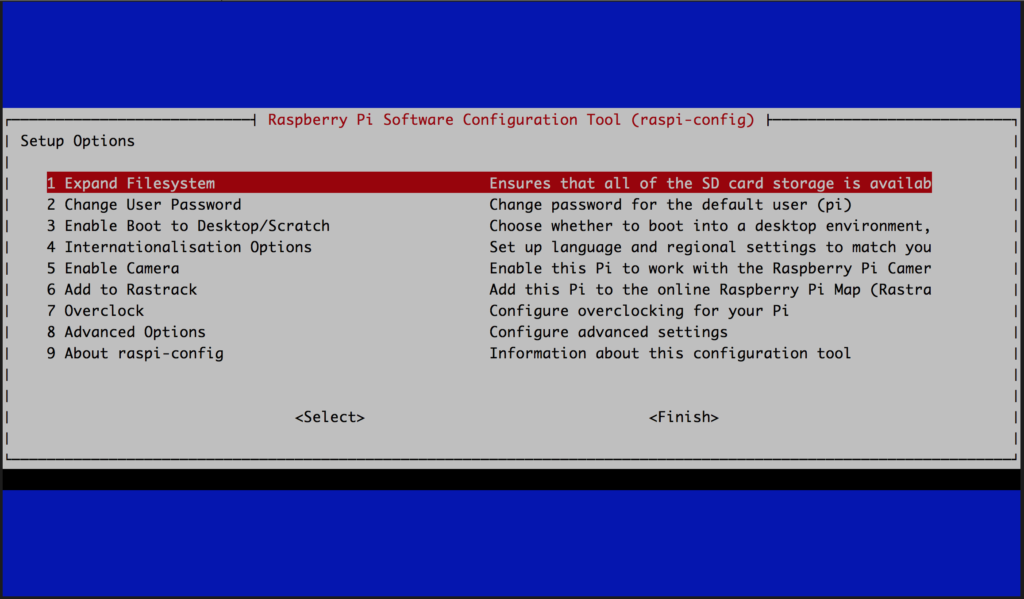
\includegraphics[scale=0.3]{Images/Raspi_config.png}
    \end{center}
    \caption{raspi-config utiliy on the Raspberry Pi}
    \label{fig:raspi_config}
\end{figure}

\subsubsection{Hardware PWM}
\paragraph{}
On Raspberry Pi board there is a lot of way to generate pwm signals.
The most of the time, these methods are software based and so they are not
accurate. With a lot of searches, we found a website who speak about the
raspberry pi's hardware pwm signals. There is apparently an hardware pwm
generator used by the bord to generate sounds. It's better to use hardware 
generated pwm, because if the processor has a slow down and the interrupt
is not correctly handled, the pwm duty cycle will not be very accurate and
the car will not be able for instance to follow a straight line, because the
bearing of the car is controled by a servomotor with a pwm signal.

\paragraph{}So we decided to use this tutorial : \cite{pi_pwm}, 
which explain us how to setup pwm signals on the Raspberry Pi,
and how to correctly configure the files to have a standard pwm signal
which is generated. Then we need to give the rights to users for reading and
writing in these files. All these bash command are in \textit{init\_pwm.sh}.

\paragraph{}
Then we have to add some automation. So we created a \textit{crontab} rule.
That will automatically create all the required files and allow the permissions
to every users. We just have to write in the file \textit{duty\_cycle} a value between
$1.000.000$ and $2.000.000$, and the Raspberry Pi will read and adjust pwm signals
in real time.

\paragraph{}
Last but not least, we setup an autologin in order to open a session automatically
when the Raspberry Pi boot. That's very usefull in order to launch our programms
easily on boot and without any keyboard, mouse or monitor.